\section{nonnative-sub}
\label{nonnative-sub}

\begin{enumerate}
    \item target
        check the substract relation among three nonnative target objects.
    \item constraints-logic
        \begin{itemize}
            \item check equation for gadget,  diff + b = a + modular * overflow
            \item check that "overflow is bool"
            \item check that "diff.limbs is range U32"
        \end{itemize}
    \item nonnative-sub process layout
        \begin{figure}[!ht]
            \centering
            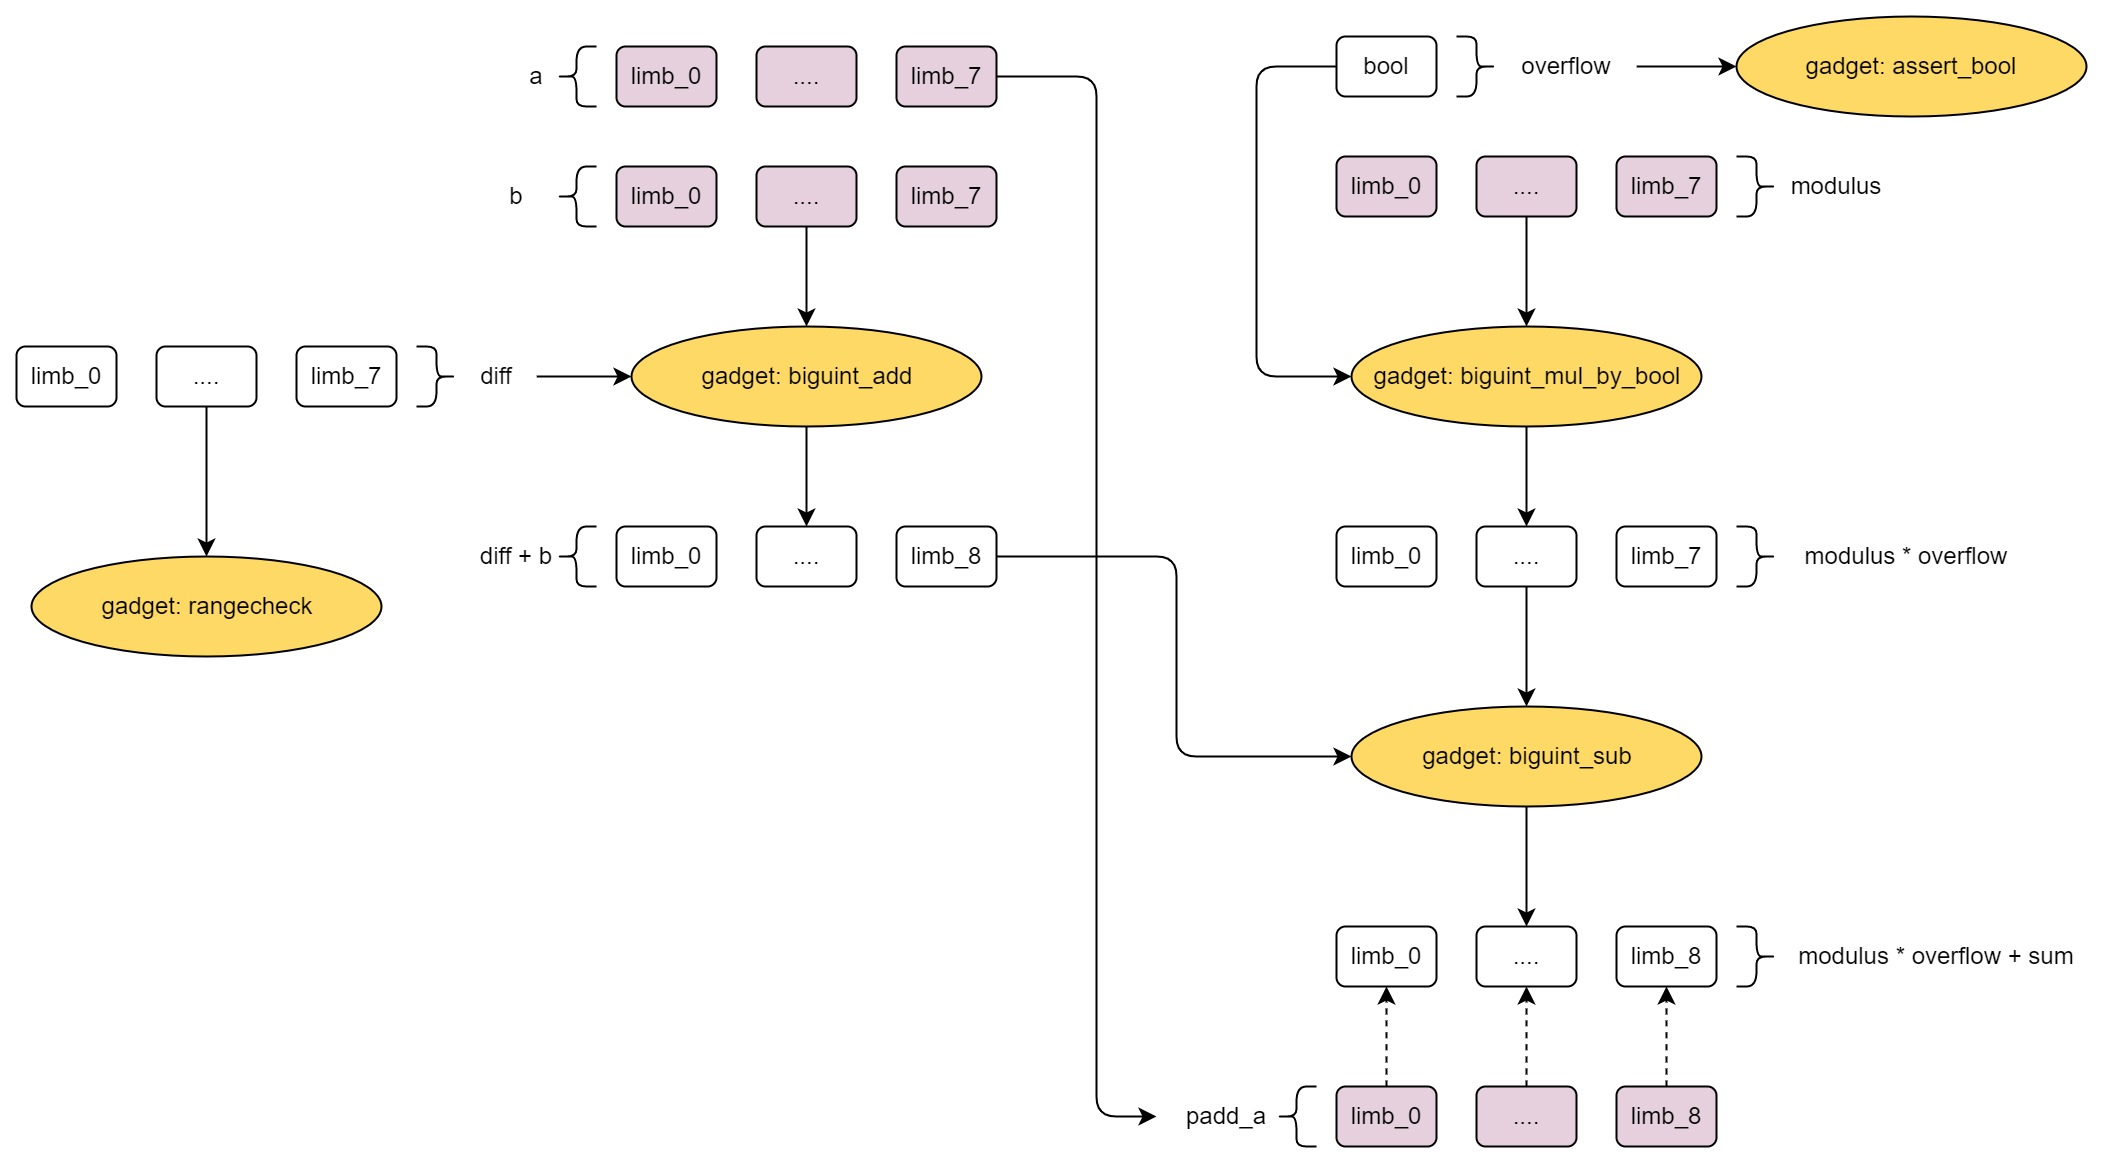
\includegraphics[width=0.8\textwidth]{nonnative-sub-layout.jpg}
            \caption{nonnative-sub layout}
            \label{fig:nonnative-sub-layout}
        \end{figure}
    
    \item constraints-info and costs
        \begin{itemize}
            \item gadget biguint-add num: 1
            \item gadget biguint-sub num: 1
            \item gadget biguint-mul-by-bool num: 1
            \item gadget u32rangecheck num: 1
            \item gadget assert-bool num: 1
            \item gate type num: 4(U32AddManyGate, U32SubtractionGate, U32RangeCheckGate, ArithmeticGate)
            \item gate instance num: 7 = 2(U32AddManyGate) + 2(U32SubtractionGate) + 1(U32RangeCheckGate) + 1(ArithmeticGate(1,0)) + 1(ArithmeticGate(1,-1))
            \item copy-constraints: 89 = 32{biguint-add num} + 27{U32SubtractionGate} + 9{biguint-mul-by-bool} + 8{u32rangecheck} + 4{assert-bool} + 9
        \end{itemize}

    \item questions
        \begin{itemize}
            \item why not constraint for overflow at nonnative-add?
            \item why not make u32rangecheck for input at nonnative-add?
        \end{itemize}

\end{enumerate}